% Standalone vector figure extracted from manuscript.tex.
% Rebuild all figures from the project root: bash tkz/build.sh
\documentclass[tikz,border=2pt,class=IEEEtran]{standalone}
\usepackage{amsmath,amssymb,amsfonts}
\usepackage{xcolor}
\usetikzlibrary{positioning,arrows.meta,calc,backgrounds}

% Match the manuscript's IEEE Access text and math font settings.
\renewcommand{\textbf}[1]{{\fontseries{b}\selectfont #1}}
\renewcommand{\textit}[1]{{\itshape #1}}
\makeatletter
\AtBeginDocument{%
  \fontencoding{T1}\rmfamily\fontseries{m}\fontsize{10}{12}\selectfont
  \gdef\operator@encoding{T1}%
  \gdef\encodingdefault{T1}}
\makeatother

% ---- shared palette for review figures ----
\definecolor{cVLA}{HTML}{34618E}   % VLA lane / policy blue
\definecolor{cWM}{HTML}{9E4A3F}    % world-model lane
\definecolor{cCONV}{HTML}{5E4B8B}  % convergence purple
\definecolor{cGood}{HTML}{3A7D44}  % verified green
\definecolor{cWarn}{HTML}{B07A2A}  % caution amber
\definecolor{cPale}{HTML}{F2F0EA}  % pale panel fill
\tikzset{
  fnode/.style={draw=black!55, fill=white, rounded corners=1.5pt,
                inner sep=2.5pt, align=center, font=\fontsize{8}{9.5}\selectfont},
  flane/.style={draw=none, rounded corners=2pt, inner sep=3pt,
                align=center, font=\fontsize{8}{9.5}\selectfont\bfseries, text=white},
  farr/.style={-{Stealth[length=2mm]}, thick, black!60},
}


\newcommand{\figfont}{\fontsize{8}{9.5}\selectfont}

\begin{document}

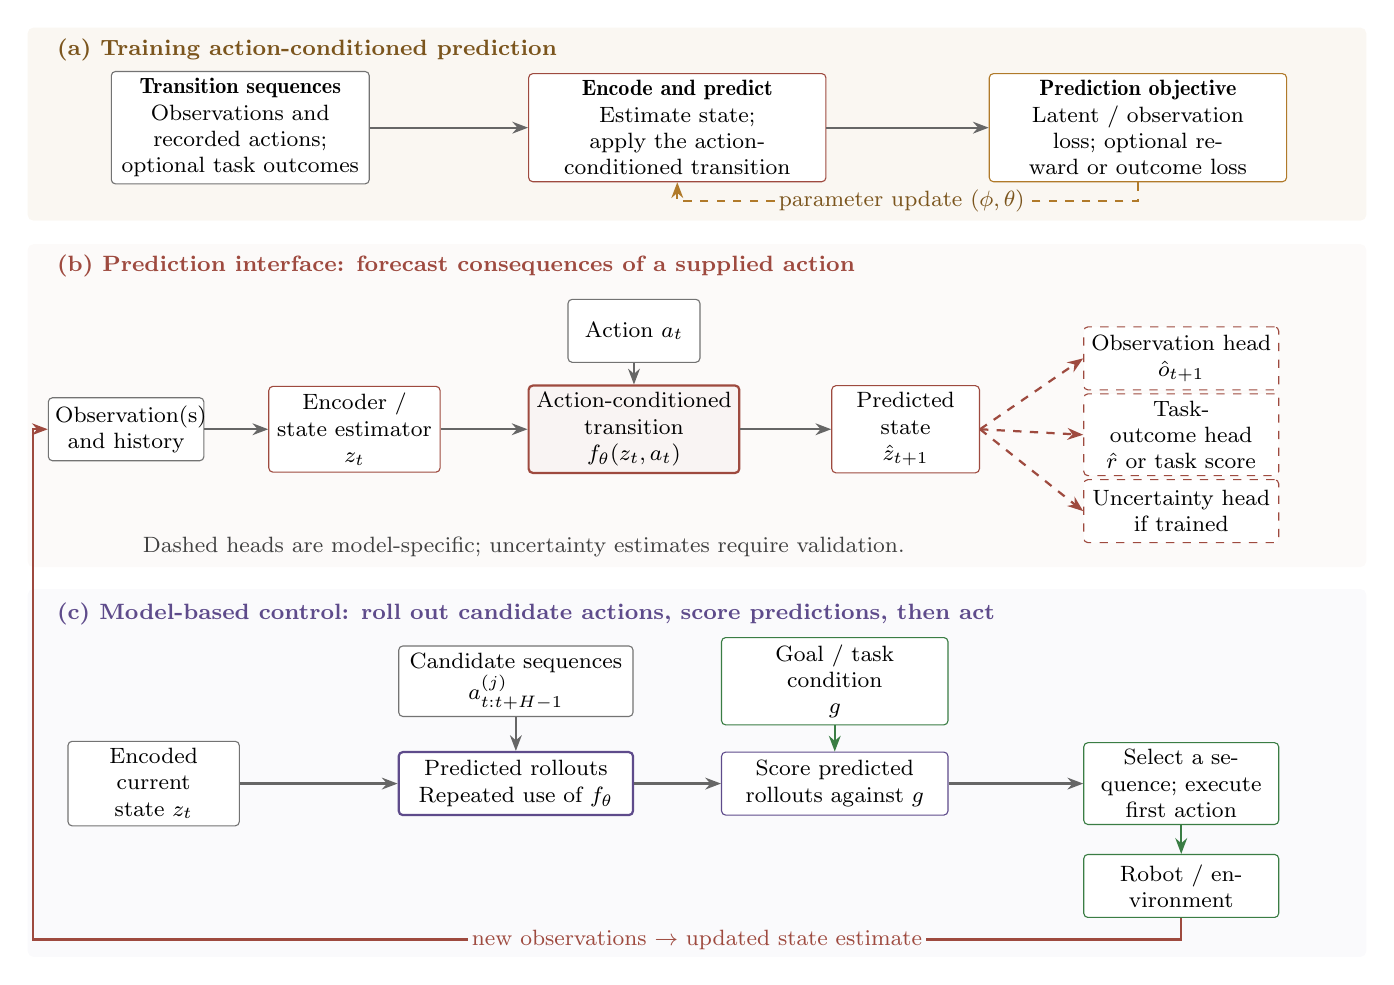
\begin{tikzpicture}[font=\figfont]
\tikzset{box/.style={fnode,minimum height=8mm},
 optional/.style={box,draw=cWM,dashed,text width=23mm},
 title/.style={font=\fontsize{8.5}{10}\selectfont\bfseries,anchor=west}}
\fill[cWarn!6,rounded corners=2pt] (0,.6) rectangle (17,3.05);
\node[title,text=cWarn!70!black] at (.25,2.77) {(a) Training action-conditioned prediction};
\node[box,text width=31mm] (data) at (2.7,1.78) {\textbf{Transition sequences}\\Observations and recorded actions; optional task outcomes};
\node[box,draw=cWM,text width=36mm] (train) at (8.25,1.78) {\textbf{Encode and predict}\\Estimate state; apply the action-conditioned transition};
\node[box,draw=cWarn,text width=36mm] (loss) at (14.1,1.78) {\textbf{Prediction objective}\\Latent / observation loss; optional reward or outcome loss};
\draw[farr] (data)--(train);\draw[farr] (train)--(loss);
\draw[farr,dashed,cWarn] (loss.south)--(14.1,.85)--(8.25,.85)--(train.south);
\node[fill=cWarn!6,inner sep=1pt,text=cWarn!70!black] at (11.1,.85) {parameter update $(\phi,\theta)$};
% The prediction interface distinguishes supplied controls from task goals.
\fill[cWM!3,rounded corners=2pt] (0,-3.8) rectangle (17,.3);
\node[title,text=cWM] at (.25,.02) {(b) Prediction interface: forecast consequences of a supplied action};
\node[box,text width=18mm] (obs) at (1.25,-2.05) {Observation(s) and history};
\node[box,draw=cWM,text width=20mm] (encoder) at (4.15,-2.05) {Encoder / state estimator\\$z_t$};
\node[box,draw=cWM,thick,fill=cWM!6,text width=25mm] (transition) at (7.7,-2.05) {Action-conditioned transition\\$f_\theta(z_t,a_t)$};
\node[box,text width=15mm] (action) at (7.7,-.8) {Action $a_t$};
\node[box,draw=cWM,text width=17mm] (future) at (11.15,-2.05) {Predicted state\\$\hat z_{t+1}$};
\draw[farr] (obs)--(encoder);\draw[farr] (encoder)--(transition);
\draw[farr] (action)--(transition);\draw[farr] (transition)--(future);
\node[optional] (decoder) at (14.65,-1.15) {Observation head\\$\hat o_{t+1}$};
\node[optional] (outcome) at (14.65,-2.12) {Task-outcome head\\$\hat r$ or task score};
\node[optional] (uncertainty) at (14.65,-3.09) {Uncertainty head\\if trained};
\foreach \headnode in {decoder,outcome,uncertainty}{\draw[farr,dashed,cWM] (future.east)--(\headnode.west);}
\node[text=black!75,align=center,text width=117mm] at (6.3,-3.55)
 {Dashed heads are model-specific; uncertainty estimates require validation.};
% One possible control use of the learned model; other uses are not asserted here.
\fill[cCONV!3,rounded corners=2pt] (0,-8.75) rectangle (17,-4.08);
\node[title,text=cCONV] at (.25,-4.4) {(c) Model-based control: roll out candidate actions, score predictions, then act};
\node[box,text width=20mm] (state) at (1.6,-6.55) {Encoded current state $z_t$};
\node[box,text width=28mm] (candidates) at (6.2,-5.25) {Candidate sequences\\$a_{t:t+H-1}^{(j)}$};
\node[box,draw=cCONV,thick,text width=28mm] (rollouts) at (6.2,-6.55) {Predicted rollouts\\Repeated use of $f_\theta$};
\node[box,draw=cGood,text width=27mm] (goal) at (10.25,-5.25) {Goal / task condition\\$g$};
\node[box,draw=cCONV,text width=27mm] (score) at (10.25,-6.55) {Score predicted rollouts against $g$};
\node[box,draw=cGood,text width=23mm] (select) at (14.65,-6.55) {Select a sequence; execute first action};
\node[box,draw=cGood,text width=23mm] (robot) at (14.65,-7.85) {Robot / environment};
\draw[farr] (state)--(rollouts);\draw[farr] (candidates)--(rollouts);
\draw[farr,cGood] (goal)--(score);\draw[farr] (rollouts)--(score);
\draw[farr] (score)--(select);\draw[farr,cGood] (select)--(robot);
\draw[farr,cWM] (robot.south)--(14.65,-8.53)--(.07,-8.53)--(.07,-2.05)--(obs.west);
\node[fill=cCONV!3,text=cWM,inner sep=1.5pt] at (8.5,-8.53) {new observations $\rightarrow$ updated state estimate};
\end{tikzpicture}
\end{document}
